\documentclass[11pt, a4paper]{article}
\usepackage{algorithmic}
%\usepackage{savesym}
%\savesymbol{IF, algorithmic}
\usepackage[utf8]{inputenc}
\usepackage[spanish]{babel}
\usepackage[paper=a4paper, left=2.4cm, right=2cm, bottom=2cm, top=2.4cm]{geometry}
\usepackage{aed2-symb}
\usepackage{textcomp}
\usepackage[section, ruled]{algorithm}
\usepackage{hyperref}
\usepackage[pdftex]{graphicx}
\usepackage{epsfig}

%\floatname{algorithm}{Algoritmo} % para que diga ``Algoritmo'' y no ``Algorithm''

\renewcommand{\algorithmiccomment}[1]{\ \ \ \textbf{//#1}} %para agregar comntarios en los algoritmos poner
% \COMMENT{ALAN ES GAY}
% \usepackage{algpseudocode}
% \usepackage{lineno}
\newenvironment{parr}
{\begin{list}{}%
         {\setlength{\leftmargin}{2em}}%
         \item[]%
}
{\end{list}}
\newcommand{\tab}{\hspace*{2em}}

\newcommand{\oper}[3]{\samepage\textsc{#1}(#2) $\rightarrow$ \textit{res} $\colon$ #3\\*}
\newcommand{\operL}[3]{\samepage\textsc{#1}(#2) $\rightarrow$ \textit{res} $\colon$ #3}
\newcommand{\operM}[2]{\samepage\textsc{#1}(#2)\\} %�sta es la operaci�n que no devuelve nada
\newcommand{\operMA}[2]{\samepage\textsc{#1}(#2)} %�sta es la operaci�n que no devuelve nada y para usar en el
%``caption'' del ``algorithm''
\newcommand{\vin}[2]{\textbf{in} \textit{#1}$\colon$#2}
\newcommand{\vinout}[2]{\textbf{in/out} \textit{#1}$\colon$#2}
\newcommand{\pre}[1]{\textbf{Pre} $\equiv$ \{#1\}\\*}
\newcommand{\post}[1]{\textbf{Post} $\equiv$ \{#1\}\\*}
\newcommand{\complej}[1]{\textbf{Complejidad:} #1\\*}
\newcommand{\desc}[1]{\textbf{Descripci\'on:} #1\\}
\newcommand{\alias}[1]{\textbf{Aliasing:} #1\\}

% \oper{nombre}{recibe}{devuelve}
% \vin{var}{tipo}
% \vinout{var}{tipo}
% \pre{}
% \post{}
% \complej{O()}
% \desc{txt}
% \alias{txt}

\newcommand{\eqobs}{$=_{obs}$}
\newcommand{\bigo}[1]{O$\big($#1$\big)$}
\newcommand{\NULL}{\textsc{Null} }
\newcommand{\aux}[3]{\samepage #1$\colon$ #2 $\rightarrow$ #3\\*}

\usepackage{hyperref}
\usepackage{color}
\usepackage{paralist}
\usepackage{multirow}
\usepackage{footnote}
\makesavenoteenv{tabular}
\usepackage{pdflscape}
\usepackage{enumitem}
\usepackage{amsmath}
\usepackage{caption}
\usepackage{subcaption}

\usepackage{lscape} 

%El siguiente paquete permite escribir la caratula facilmente
\usepackage{caratula}
\hypersetup{
  pdftitle={ Métodos Numéricos - TP2 },
  colorlinks,
  citecolor=black,
  filecolor=black,
  linkcolor=black,
  urlcolor=black 
}



\newlength{\AnchoEncabezados}\setlength{\AnchoEncabezados}{6em}
\newcommand{\EncabezadoInline}[2]{
    
    \setlength{\hangindent}{\tadAnchoEncabezados + \parindent}%
    
        \parbox{\AnchoEncabezados}{\textbf{#1}}#2%
}



\newcommand{\Encabezado}[2]{%
    \par\EncabezadoInline{#1}{#2}\par%
}

\newcommand{\funcion}[2]{\textbf{#1}{#2}\BlankLine}


%\newcommand{\myFuncion}[3]{
%	\begin{algorithm}[H][H]
%	\dontprintsemicolon
%	{\bf {#1}} {#2}\;
%	\nocaptionofalgo
%	\Indp
%	{#3}
%	\Indm
%	\BlankLine
%	\end{algorithm}
%}
   
%Datos para la caratula
\materia{Métodos Numéricos}

\titulo{TP 2 - Tu cara me suena...}

%\fecha{DDDD dd de MMMM, AAAA}

\grupo{Grupo 2}

\integrante{Franco Bartalotta}{}{franco.bartalotta@hotmail.com}
\integrante{Fernando Gasperi Jabalera}{56/09}{fgasperijabalera@gmail.com}
\integrante{Ana Sarri\'es}{144/02}{abarloventos@gmail.com}

\resumen{En este trabajo práctico, desarrollamos un método para el reconocimiento de caras basado en el enfoque de \textit{eigenfaces}. Para ello, manipulamos la base de imágenes de entrenamiento matricialmente; obteniendo las componentes principales (autovectores) de su matriz de covarianzas a través del método de la potencia con deflación. Exploramos algunos métodos de clasificación, su tasa de efectividad y su relación con posibles variaciones en el conjunto inicial de entrenamiento.}
\claves{Face Recognition, Componentes Principales, SVD}

\begin{document}
 
 %esto construye la caratula
 \maketitle
 \tableofcontents

\newpage

\section{Introducción Teórica}
%Contendrá una breve explicación de la base teórica que fundamenta los métodos involu-
%crados en el trabajo, junto con los métodos mismos. No deben incluirse demostraciones
%de propiedades ni teoremas, ejemplos innecesarios, ni definiciones elementales (como
%por ejemplo la de matriz simétrica). En vez de definiciones básicas es conveniente citar
%ejemplos de bibliografía adecuada. Una cita vale más que mil palabras.
%
El objetivo principal de este trabajo es desarrollar un método que nos permita identificar personas en tiempo real a partir de sus rostros con el máximo grado de efectividad posible.
\newline
\par
\textbf{El enfoque utilizado es el propuesto en \cite{eigenfaces} cuya característica distintiva respecto de otros enfoques es que se basa en la teoría de la información.} Bajo el supuesto de que el reconocimiento facial puede hacerse a partir de fotografías 2-D, y contando con un conjunto inicial -que llamaremos de entrenamiento- de imágenes pertenecientes al universo de rostros que se pretende reconocer, el enfoque propone trabajar con una transformación de ese espacio que permita reducir su dimensionalidad considerablemente, conservando, a la vez, la capacidad de distinguir a los elementos que viven en él.
\newline
\par
Primero se calcula la matriz de covarianza de las imagenes de entrenamiento. EXPLICAR PORQUE Y QUE ES LA MATRIZ DE COVARIANZA SIRVE, CERO DE PROBA. Una vez obtenida la matriz de covarianzas se hallana las componentes principales de dicha matriz para reducir la dimensión del espacio en que trabajermos y reducir los tiempos de cómputo. Para esto es necesario hallar los autovalores de mayor módulo y sus autovectores asociados. Dichos autovalores son necesarios ya que al reducir el espacio, naturalmente se pierde información, EXPLICAR MEJOR ESTO: los autovalores de menor módulo contienente menos información y por lo tanto es más confiable descartalos sin perder efectividad al identificar las caras.
\newline
Para obtener los autovalores aproximados (y sus respectivos autovectores) de la matriz de covarianzas se utiliza el método de la potencia combinado con deflación. Este método arrastra error al calcular un nuevo autovalor, por lo que no resulta práctico utilizarlo para calcular todos los autovalores, afortunadamente, solamente estamos interesados en los primeros y más importantes.
Una vez obtenidos los autovectores y autovalores, podemos calcular las primeras componentes de imagen vectorizada para reducir la dimensión del espacio a trabajar.
\newline
Por último hay que identificar las caras que vayan apareciendo en el sistema, para esto se vectoriza y normaliza la imagen de la cara para posteriormente quedarnos con las primeras componentes de dicha imagen, y simplemente se utiliza algún criterio basado en  distancias entre la imagen a identificar y el resto de las imagenes.


\newpage
\section{Desarrollo}
%Deben explicarse los métodos numéricos que utilizaron y su aplicación al problema
%concreto involucrado en el trabajo práctico. Se deben mencionar los pasos que si-
%guieron para implementar los algoritmos, las dificultades que fueron encontrando y la
%descripción de cómo las fueron resolviendo. Explicar también cómo fueron planteadas
%y realizadas las mediciones experimentales. Los ensayos fallidos, hipótesis y conjeturas
%equivocadas, experimentos y métodos malogrados deben figurar en esta sección, con
%una breve explicación de los motivos de estas fallas (en caso de ser conocidas).
\subsection{La implementación y algunas decisiones de diseño}
La implementación consta de 2 fases. Primero está la fase de entrenamiento:
\begin{enumerate}
 \item se obtiene la matriz $I\in\mathbb{R}^{n \times m}$ a partir de todas las imágenes de la base de entrenamiento. Para $i = 1,...,n$, llamamos $x_i$ a
 la i-ésima fila de $I$ que se corresponde con la i-ésima imagen de nuestra base vectorizada por filas. Cada posición de $x_i$ se 
 corresponde con un pixel de la imagen a la cual corresponde. Además, sabemos que $n = nimgp * \#sujetos$, siendo $nimgp$ la cantidad de imágenes
 que tengo por cada sujeto y $\#sujetos$ la cantidad de sujetos distintos a los que pertencen las imágenes de mi base de entrenamiento, y 
 $m = alto * ancho$, siendo $alto$ y $ancho$ los respectivos anchos y altos de las imágenes medidos en pixeles.
 
 \item se calcular la matriz $A$ a partir de la matriz $I$. Sus dimensiones son iguales. Obtenemos el vector $\mu = (x_1+...+x_n)/n$ que es 
 el promedio de las imágenes. Para calcular $A$, en primer lugar restamos a cada una de las filas de $I$ el vector $\mu$. Obtenemos $I'$ que contiene en la
 i-ésima fila al vector $(x_i - \mu)^t$. En segundo lugar obtenemos $A$ como: $A = I' * \sqrt{n-1}$.
 
 \item calculamos la matriz de covarianzas $M_x = A^t*A$. (Para este punto y el siguiente efectuamos un análisis alternativo que se puede ver en \ref{metodoAlternativo})
 
 \item aplicamos el método de la potencia con deflación $k$ veces sobre la matriz $M_x$. $k$ es el número de componentes principales que nos 
 interesa obtener. Conseguimos una matriz $B\in\mathbb{R}^{m \times k}$ cuya columna $b_i$ se corresponde con el autovector $a_i$ de la matriz
 $M_x$ asociado al autovalor $\lambda_i$ tal que $\lambda_1 < \lambda_2 < ... < \lambda_k \leq \lambda_{k+1} \leq ... \leq \lambda_m$. Esto es así
 por que el método de la potencia, si encuentra un autovalor, es el de mayor módulo. \cite{burden}.
 
 \item aplicamos la transformación característica a todas las imágenes de nuestra base de entrenamiento. La transformación característica
 de $x_i$ está dada por \begin{displaymath}
			    tc(x_i) = ({b_1^t}x_i, {b_2^t}x_i,..., {b_k^t}x_i)\in\mathbb{R}^k
                        \end{displaymath}
\end{enumerate}
y luego está la fase de identificación en la que recibimos una nueva imagen e identificamos a qué sujeto pertenece:
\begin{enumerate}
 \item recibimos la imagen y la vectorizamos por filas de la misma forma que lo hicimos con las imágenes en nuestra base de entrenamiento
 en la primera fase y obtenemos $x_{identificar}$.
 
 \item calculamos su transformación característica de la misma manera que lo hicimos en la fase de entrenamiento y con la misma matriz $B$
  \begin{displaymath}
			    tc(x_{identificar}) = ({b_1^t}x_{identificar}, {b_2^t}x_{identificar},..., {b_k^t}x_{identificar})\in\mathbb{R}^k
  \end{displaymath}
 
 \item decidimos a cuál sujeto pertenece por alguno de los dos métodos que describimos más adelante.
\end{enumerate}
Los métodos que implementamos para decidir a qué sujeto pertenece una imagen luego de haber calculado su transformación
característica son los siguientes:
\begin{description}
  \item[Distancia mínima] calculamos la distancia entre la transformación característica de la imagen que queremos identificar
  y todas las imágenes de nuestra base. Decidimos que la imagen nueva corresponde al sujeto al cual pertenece la imagen cuya transformación
  característica es la más cercana a la transformación característica de la nueva imagen. Es decir, con el de distancia mínima.
  \item[Distancia mínima al promedio] calculamos el promedio de las distancias entre la transformación característica de la imagen que 
  queremos identificar y las imágenes de cada uno de nuestros sujetos. De esta forma obtenemos una distancia promedio a los diferentes sujetos.
  Finalmente, decidimos que la imagen nueva corresponde al sujeto al cual pertenece el promedio de distancias más cercano 
  a la transformación característica de la nueva imagen.
\end{description}
Aclaramos que el método de la potencia que implementamos recibe como vector inicial $b_0 = (1,...,1)$.
\par
La técnica de deflación arrastra el error generado por el método de la potencia, haciendo que los últimos autovalores tengan un error 
de cálculo mayor que los primeros. Este problema es mitigado por el hecho de que sólo tomamos los $k$ mayores pero de todas formas 
probablemente quede reflejado en la experimentación. Además, tomamos $iter = 300$ en la implementación del método de la potencia, el
máximo para que los tiempos de cómputo se mantuvieran en un rango aceptable, para obtener mayor precisión en el cálculo de los autovalores
y así compensar el error arrastrado por la deflación.

\subsection{Elección conveniente de la matriz de covarianzas para imágenes grandes}

El método alternativo consiste en hallar una relación entre los autovalores y autovectores de $B = A^tA$, y los autovectores y autovalores de $C = A A^t$.
Veamos primero como se escribe la matriz $C$. Si consideramos la descomposición en valores singulares de la matriz $A$:
\begin{displaymath}
  C = U \Sigma V^t (U \Sigma V^t)^{t} = U \Sigma V^t V \Sigma^{t} U^{t}  = U \Sigma \Sigma^{t} U^{t}
\end{displaymath}
De esta manera encontramos la forma $SVD$ de la matriz $C$. Y en consecuencia podemos intuir que $U^t$ contiene los autovectores de $C$ en sus columnas.
Pasemos a confirmar la hipótesis anterior, sabemos que $u_{i} = \frac{1}{\theta_{i}}Av_{i}$ con $\theta_{i} = \sqrt{ \lambda_{i} }$, y que $A^{t} A v_{i} = \lambda_{i} v_{i}$, por lo tanto:
\begin{displaymath}
C u_{i} = A A^{t} u_{i} = \frac{1}{ \theta_{i} } A A^{t}  A v_{i} =  \frac{ 1 }{  \theta_{i} } A  \lambda_{i} v_{i} =  \lambda_{i} \frac{ 1 }{ \theta_{i} } A  v_{i} = \lambda_{i} u_{i}.
\end{displaymath}
De lo anterior se deduce directamente que $\lambda_{i}$ es el autovalor asociado al autovector $u_{i}$ para la matriz $C$.
Veamos cómo se puede hallar $v_{i}$ conociendo $u_{i}$:
\begin{displaymath}
  u_{i} = \frac{1}{ \theta_{i} } A v_{i}
\end{displaymath}
multiplicando por $A^{t}$ en ambos lados se obtiene:
\begin{displaymath}
  A^{t} u_{i} =  \frac{1}{ \theta_{i} } A^{t} A v_{i},  
\end{displaymath}
que es igual a: 
\begin{displaymath}
  A^{t} u_{i} = \frac{\lambda_{i}}{ \theta_{i} }  v_{i} 
\end{displaymath}
despejando y reemplazando $\theta_{i}$:
\begin{displaymath}
  \frac{ \sqrt{\lambda_{i} } }{ \lambda_{i} }  A^{t} u_{i} = v_{i}
\end{displaymath}
De lo anterior podemos describir el siguiente método para hallar los autovectores de $B = A^{t}A$:
\begin{enumerate}
\setlength{\itemindent}{0.2in}
\item Calcular $C = AA^{t}$.
\item Mediante el método de la potencia hallar los autovectores y autovalores de $C$, notar que los autovalores coinciden para ambas matrices, por lo que si  se podía utilizar el método para $B$, también se puede hacer para $C$.
\item Para cada autovector $u_{i}$ hallado, lo multiplico por $\frac{ \sqrt{\lambda_{i} } }{ \lambda_{i} }  A^{t}$ para obtener $v_{i}$.
\end{enumerate}



%\subsection{Elección conveniente de la matriz de covarianzas para imágenes grandes}
\label{metodoalternativo}
El método alternativo consiste en utilizar la matriz $A.A^t$ en lugar de la matriz $A^tA$ a la hora de calcular los autovectores de la transformación característica. 
\par
Esto resulta posible, si advertimos que ambas matrices poseen los mismos autovalores. Veamos la demostración:
\par
Sea $u_{i}$ autovector de $A.A^{t}$ asociado a $\lambda_{i}$, entonces tenemos que:
\begin{displaymath}
  (A.A^{t}).u_{i} = \lambda_{i}.u_{i},  
\end{displaymath}
\par
multiplicando por $A^{t}$ a ambos lados de la igualdad, resulta:
\begin{displaymath}
  A^{t}.(A.A^{t}).u_{i} = A^{t}\lambda_{i}.u_{i},  
\end{displaymath}

que por propiedad de matrices y escalares, resulta:
\begin{displaymath}
 (A^{t}.A).(A^{t}.u_{i}) = \lambda_{i}.(A^{t}.u_{i}),  
\end{displaymath}
Y observando esta última igualdad, notamos que llamando $v_{i}$ a $A^{t}.u_{i}$ entonces $v_{i}$ resulta autovector de $A^{t}.A$ asociado a $\lambda_{i}$.
\par
De lo anterior, se desprende que todo autovalor de $A.A^{t}$ también lo es de $A^{t}.A$ (y tomando $A=A^{t}$ obtendríamos la vuelta). Este resultado nos permite elegir el producto de matrices que viva en un espacio de menor dimensión, y calcular sobre él, el método de la potencia, sabiendo que hallaremos los mismos autovalores.
\par
Además, la última línea de la demostración también nos indica cuál será el método para calcular el autovector asociado: $v_{i}=A^{t}.u_{i}$.



\subsection{Comparación de la complejidad de los métodos}
El método 1 trabaja con la matriz $AA^t$ y el método 2 trabaja con la matriz $A^tA$.
La matriz $A\in\mathbb{R}^{n \times m}$ con $m = pixels(img)$ y $n = nimgp * \#personas$. Por lo tanto $A^t\in\mathbb{R}^{m \times n}$.
Por lo tanto tenemos que $AA^t\in\mathbb{R}^{n \times n}$ y $A^tA\in\mathbb{R}^{m \times m}$.

En el \'unico punto que divergen los algoritmos es en el c\'alculo de los $k$ mayores autovalores, y sus
autovectores asociados, de $M_x = A^tA$, la matriz de covarianza. 
El m\'etodo 1 aplica el m\'etodo de la potencia con deflaci\'on directamente sobre la matriz $M_x$. 
El m\'etodo 2 primero aplica el m\'etodo de la potencia sobre la matriz $M^t_x = AA^t$. Luego

\subsection{Algoritmos}

% MÉTODO DE LA POTENCIA
\begin{algorithm}[!h]
\caption{metodoDeLaPotencia(Matriz $A$, Vector $v$, Int $iter$)}
\label{pseudo:metodoDeLaPotencia}
\begin{algorithmic}
  \FOR {$i=1$ hasta $iter$}
    \STATE $y = Ax$
    \STATE $x = \frac{y}{\parallel y \parallel}$
  \ENDFOR
\end{algorithmic}
\end{algorithm}
% DEFLACIÓN
\begin{algorithm}[!h]
\caption{deflacionar(Matriz $A$, Vector $autovector$, Double $\lambda$)}
\label{pseudo:deflacionar}
\begin{algorithmic}
  \STATE $V = vv^t$
  \STATE $B = A - \lambda V$
\end{algorithmic}
\end{algorithm}
% DESPEJE DE LOS AUTOS DE AtA TENIENDO LOS DE AAt
\begin{algorithm}[!h]
\caption{despejar(Matriz $A$, Vector $v$, Double $\lambda$)}
\label{pseudo:despejar}
\begin{algorithmic}
  \STATE $u$ = $v\frac{ \sqrt{\lambda_{i} } }{ \lambda_{i} }  A^{t}$   
\end{algorithmic}
\end{algorithm}
% IDENTIFICAR CARA - DISTANCIA MÍNIMA
\begin{algorithm}[!h]
\caption{identificarDistanciaMinima(Vector $tc_{nueva}$, Matriz $TC$)}
\label{pseudo:identificarDistanciMinima}
\begin{algorithmic}
  \FOR {$i=1$ hasta $\#filas(TC)$}
    \STATE $tc_{base}$ = $fila(i, TC)$
    \STATE $diff$ = $tc_{nueva}$ - $tc_{base}$
    \STATE $dist$ = $norm(diff)$
    \IF{ $i == 1$ }
      \STATE $minimo$ = $dist$
    \ENDIF
    \IF{ $dist < minimo$ }
      \STATE $minimo$ = $dist$
    \ENDIF    
  \ENDFOR
\end{algorithmic}
\end{algorithm}
% IDENTIFICAR CARA - DISTANCIA EN PROMEDIO MÍNIMA
\begin{algorithm}[!h]
\caption{identificarDistanciaPromedioMinima(Vector $tc_{nueva}$, Matriz $TC$, Int $iSujetos$, Int $nimgp$)}
\label{pseudo:identificarDistanciaPromedioMinima}
\begin{algorithmic}
  \FOR {$i=1$ hasta $iSujetos$}
    \STATE $acum$ = $0$
    \FOR {$j=1$ hasta $nimgp$}    
      \STATE $tc_{base}$ = $fila(nimgp*i+j, TC)$
      \STATE $diff$ = $tc_{nueva}$ - $tc_{base}$
      \STATE $acum$ += $norm(diff)$      
    \ENDFOR
    \STATE $iDistanciaPromedio$ = $\frac{acum}{nimgp}$
    \STATE agregar($iDistanciaPromedio$, $aDist$)
  \ENDFOR
  \STATE $sujeto$ = min($aDist$)
\end{algorithmic}
\end{algorithm}
\FloatBarrier
\subsection{Tests}
En esta sección haremos una introducción a las experimentaciones que decidimos realizar.
\subsection{Cantidad de componentes princiaples VS tasa de efectividad}
El objetivo de la siguiente experimentación es analizar como afecta el n\'umero de componentes principales utilizado a la tasa de efectividad
que obtenemos al identificar sujetos. Las variables a considerar son: 
personas = 40
sujetos a identificar = 1 imagen por persona
resolución = 112x92
componentes= 1-19 +3
5 al azar por cada componente principal y después tomo el promedio

\subsection{Comparación de la de la tasa de eficiencia en función de la cantidad de personas}
En este experimento se intenta analizar como influye la cantidad de personas en la tasa de eficiencia del reconocimiento de imágenes. Para esto vamos a concentrarnos solo en la variable de la cantidad de personas por lo que hay que fijar el resto de los parámetros en sus valores óptimos. La experimentación se va a hacer sobre la base de imágenes grandes, con cinco imágenes por persona (valor generoso pero dentro de los límites reales), y con quince componentes principales y con la técnica de reconocimiento más efectiva.

Se espera que cuantas más personas haya (y en consecuencia más imágenes), la probablidad de que haya imagénes similares de distintas personas o incluso personas similares es más alta, por lo que tasa de reconocimiento va a ser menor.

\subsubsection{nimgp vs Tasa de efectividad}
En la siguiente experimentación queremos analizar cómo afecta a la efectividad la cantidad de imágenes que tomamos por sujeto, $nimgp$, para la base
de entrenamiento a la tasa de efectividad. La base total con la que contamos contiene 41 sujetos y 10 fotos por cada uno de ellos. Es una base que
consideramos pequeña por lo cual vamos a intentar abarcar la mayor cantidad de combinaciones posibles de $nimgp$ y las fotos que tomamos de
entrenamiento con las de test.
¿Cómo vamos a variar las variables?
¿Qué esperamos obtener?
¿Por qué es interesante realizar este test?
¿Qué desventajas tenemos con la base dada?

personas = 40
sujetos a identificar = restantes
resolución = 112x92
componentes= 15, 30, 45
20 al azar por cada cantidad de caras y después tomo el promedio
caras que tomo por persona=1,9
\subsubsection{Resolución de las imágenes vs Tasa de efectividad}
En esta experimentación se analizará la tasa de efectividad en función de la la resolución de las imágenes utilizadas. Para esto se utilizaron 5 escenarios posibles que corresponden a diferentes configuraciones de los parámetros. De esta manera se definen las distintas condiciones del experimento en:
\begin{itemize}
\item Peśima: Se utilizan 10 componentes y 1 imagen por persona.
\item Mala: Se utilizan 10 componentes y 3 imágenes por persona.
\item Regular: Se utilizan 15 componentes y 5 imágenes por persona.
\item Buena: Se utilizan 30 componentes y 7 imágenes por persona.
\item Excelente: Se utilizan 30 componentes y 9 imágenes por persona.
\end{itemize}
La cantidad de personas se fijó en $41$ ya que este parámetro no modifica la condición de los escenarios tanto como los otros dos. Se realizaron varias experimentaciones para cada escencario y para cada resolución tomando imágenes al azar para cada sujeto. El método de identificación utilizado fue el de distancia mínima por que es el más efectivo. Este experimento intenta probar como afecta la resolución de las imágenes a la tasa de efectividad. Es natural pensar que cuanto mayor sea la resolución más información tendrán las imágenes por lo que resultados serán más exactos.

\subsubsection{Comparación de los métodos de identificación}
La siguiente experimentación tiene por objetivo comparar la tasa de efectividad entre el método de identificación por distancia mínima
y el método de identificación por distancia promedio mínima. Además, nos interesa determinar si la combinación óptima, en términos de 
la tasa de efectividad obtenida, es la misma para los dos métodos de identificación. Correremos los tests con las mismas variables que
en la primera experimentación pero aplicando el método de identificación por distancia promedio mínima para la fase de identificación.


\newpage
\section{Resultados}
%Deben incluir los resultados de los experimentos, utilizando el formato más adecuado
%para su presentación. Deberón especificar claramente a qué experiencia corresponde
%cada resultado. No se incluirán aquí corridas de máquina. Algo fundamental en su
%aprendizaje en la materia es la presentación de resultados de forma clara y concisa para
%el lector.

% TASA DE EFICIENCIA EN FUNCIÓN DE LA CANTIDAD DE COMPONENTES PRINCIPALES TOMADAS
\subsection{Test de tasa de eficiencia en función de la cantidad de componentes principales consideradas}
\begin{figure}[H]{}
\centering
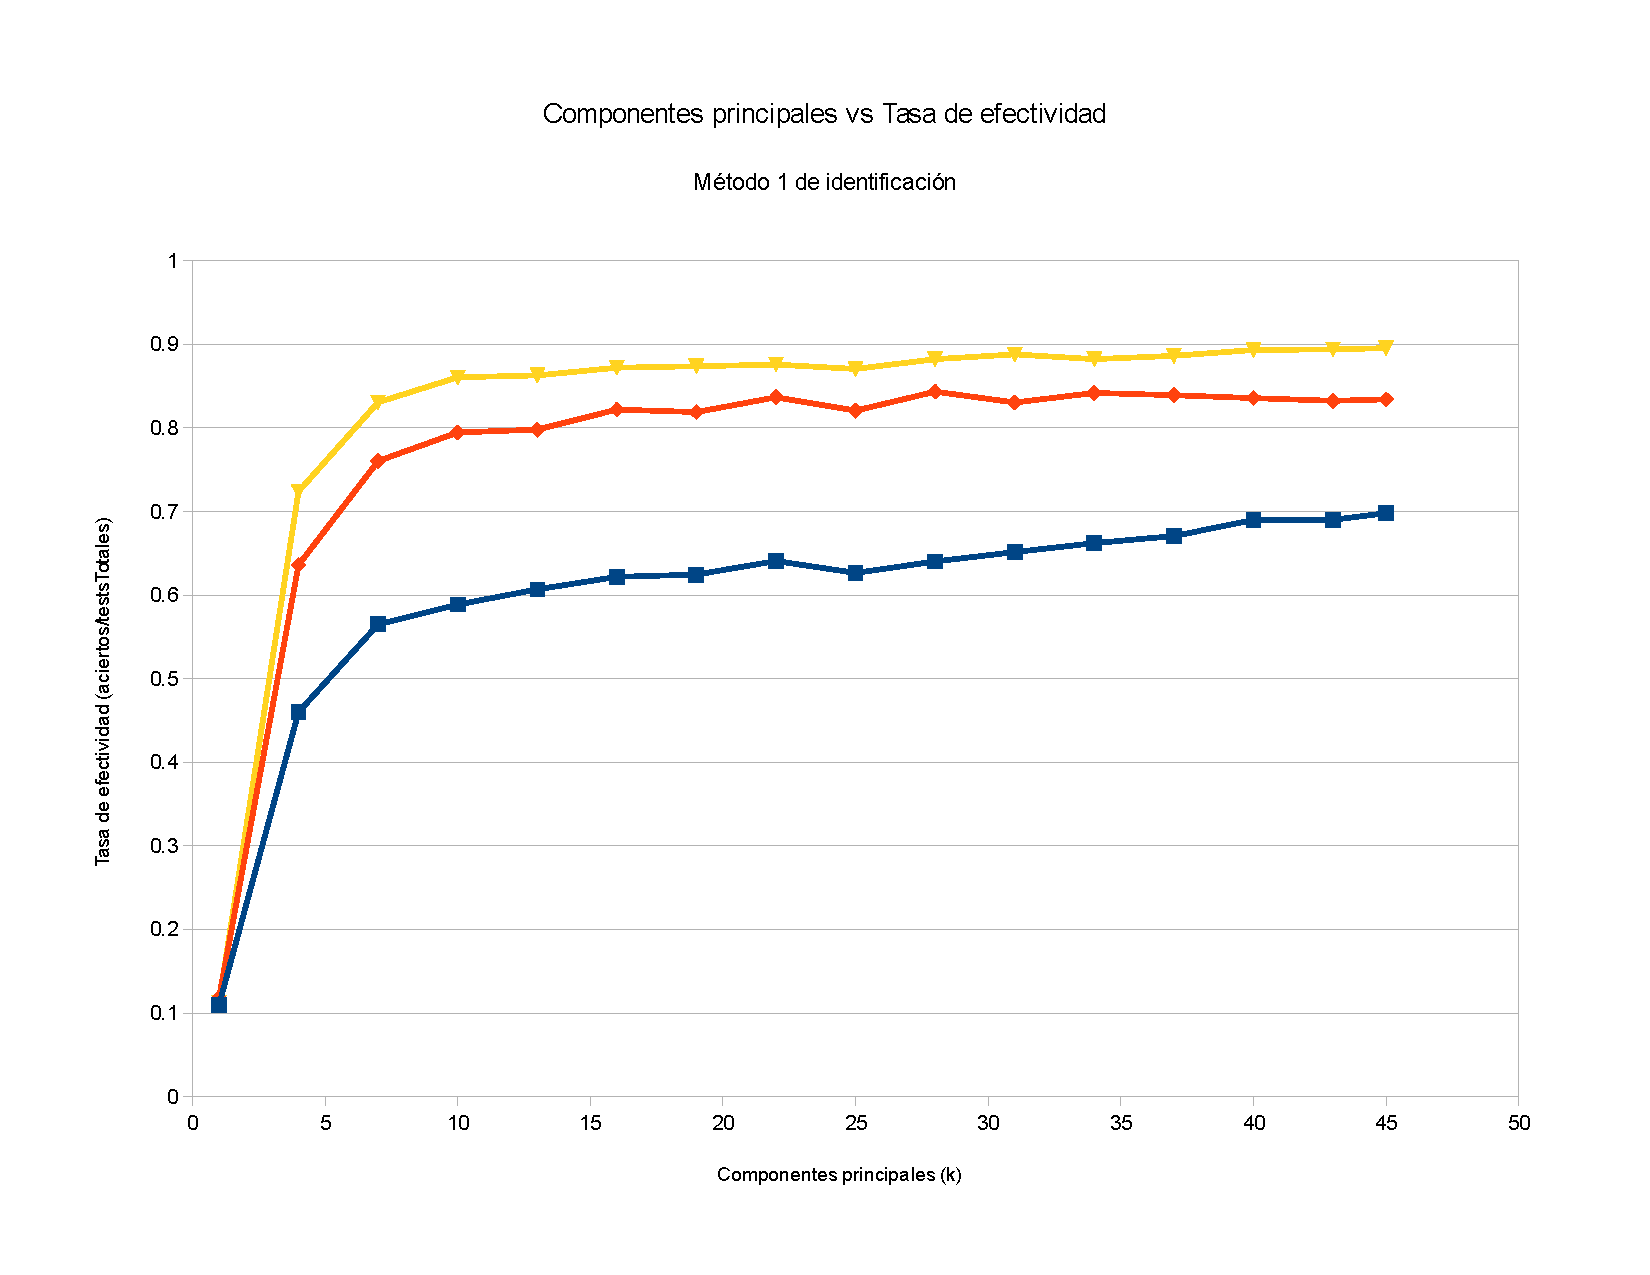
\includegraphics[scale=0.5]{graphs/componentesPrincipalesVsTasaDeEfectividadM1.pdf}
\caption{El método 1 de identificación se corresponde con el de Distancia Mínima}
\label{CPvsTE}
\end{figure}

Línea azul: $nimgp = 3$. Línea roja: $nimgp = 6$. Línea amarilla: $nimgp = 9$.

% TASA DE EFICIENCIA EN FUNCIÓN DE LA CANTIDAD DE SUJETOS CONSIDERADOS
\subsection{Test de tasa de eficiencia en función de la cantidad de personas}
\begin{figure}[H]{}
\centering
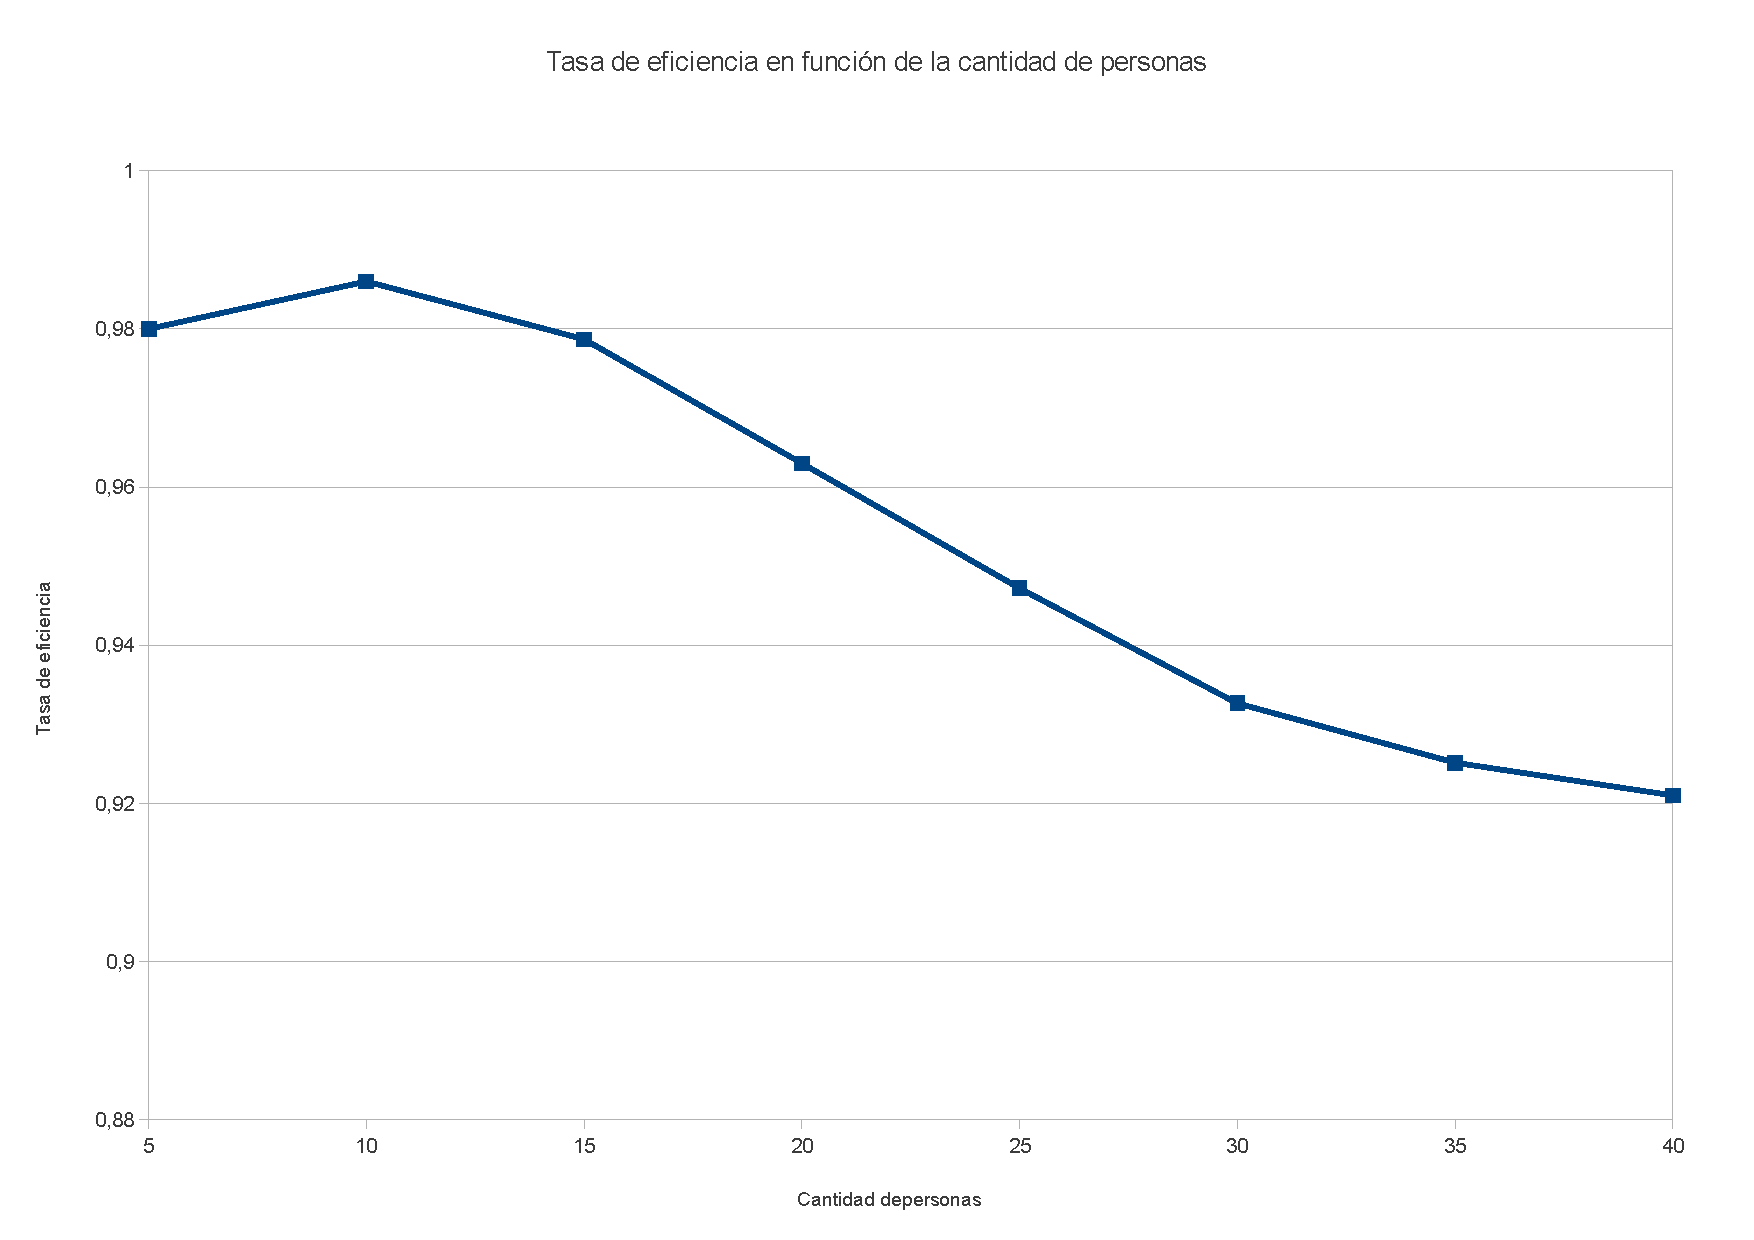
\includegraphics[scale=0.5]{graphs/CPvsTE.pdf}
\caption{Tasa de eficiencia en función de la cantidad de personas.}
\label{CPvsTE}
\end{figure}

% TASA DE EFICIENCIA EN FUNCIÓN DE nimgp
\subsection{Test de tasa de eficiencia en función de nimgp}
\begin{figure}[H]{}
\centering
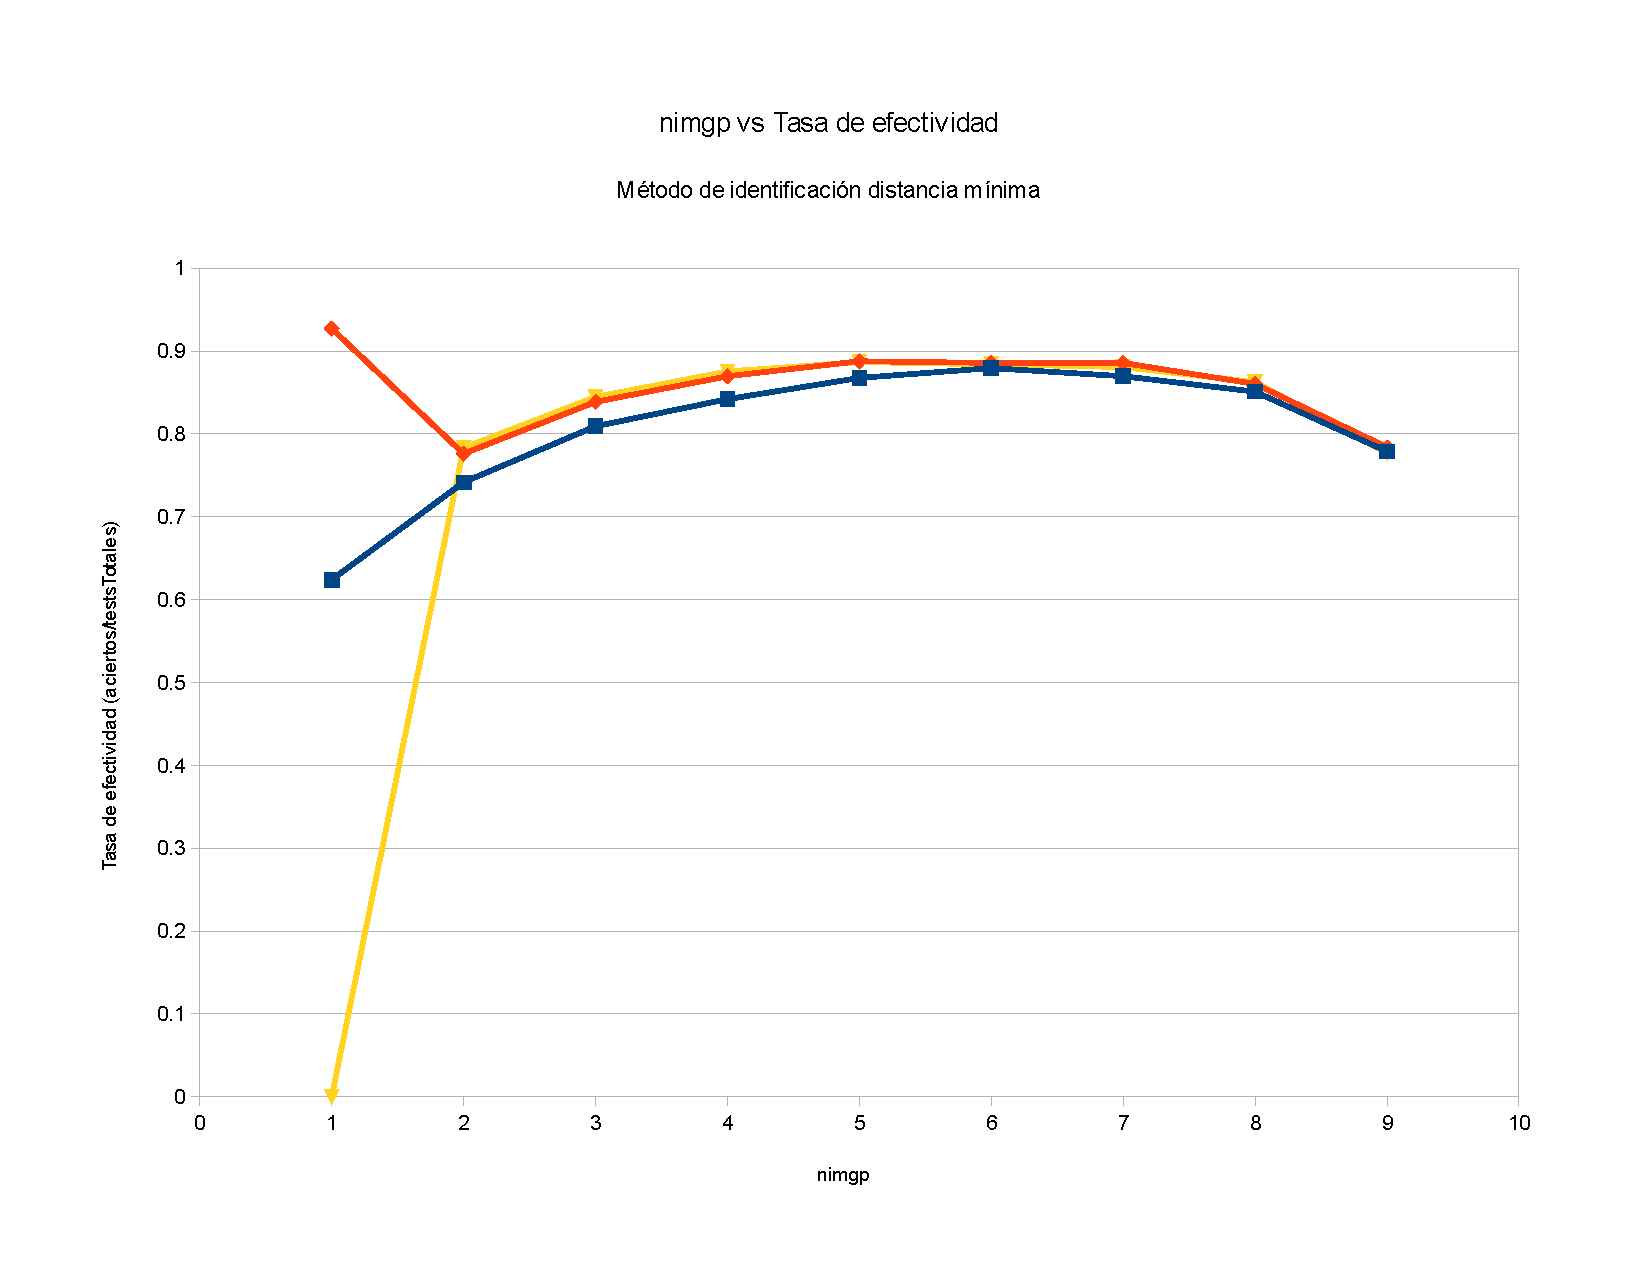
\includegraphics[scale=0.5]{graphs/nimgpVsTasaDeEfectividad.pdf}
\caption{Se graficó para 15, 30 y 45 componentes principales}
\label{nimgpvsTE}
\end{figure}

Línea azul: $k = 15$. Línea roja: $k = 30$. Línea amarilla: $k = 45$.

% TASA DE EFICIENCIA EN FUNCIÓN DE LA CANTIDAD DE COMPONENTES PRINCIPALES TOMADAS
\subsection{Test de comparación de los métodos de identificación}
\begin{figure}[H]{}
\centering
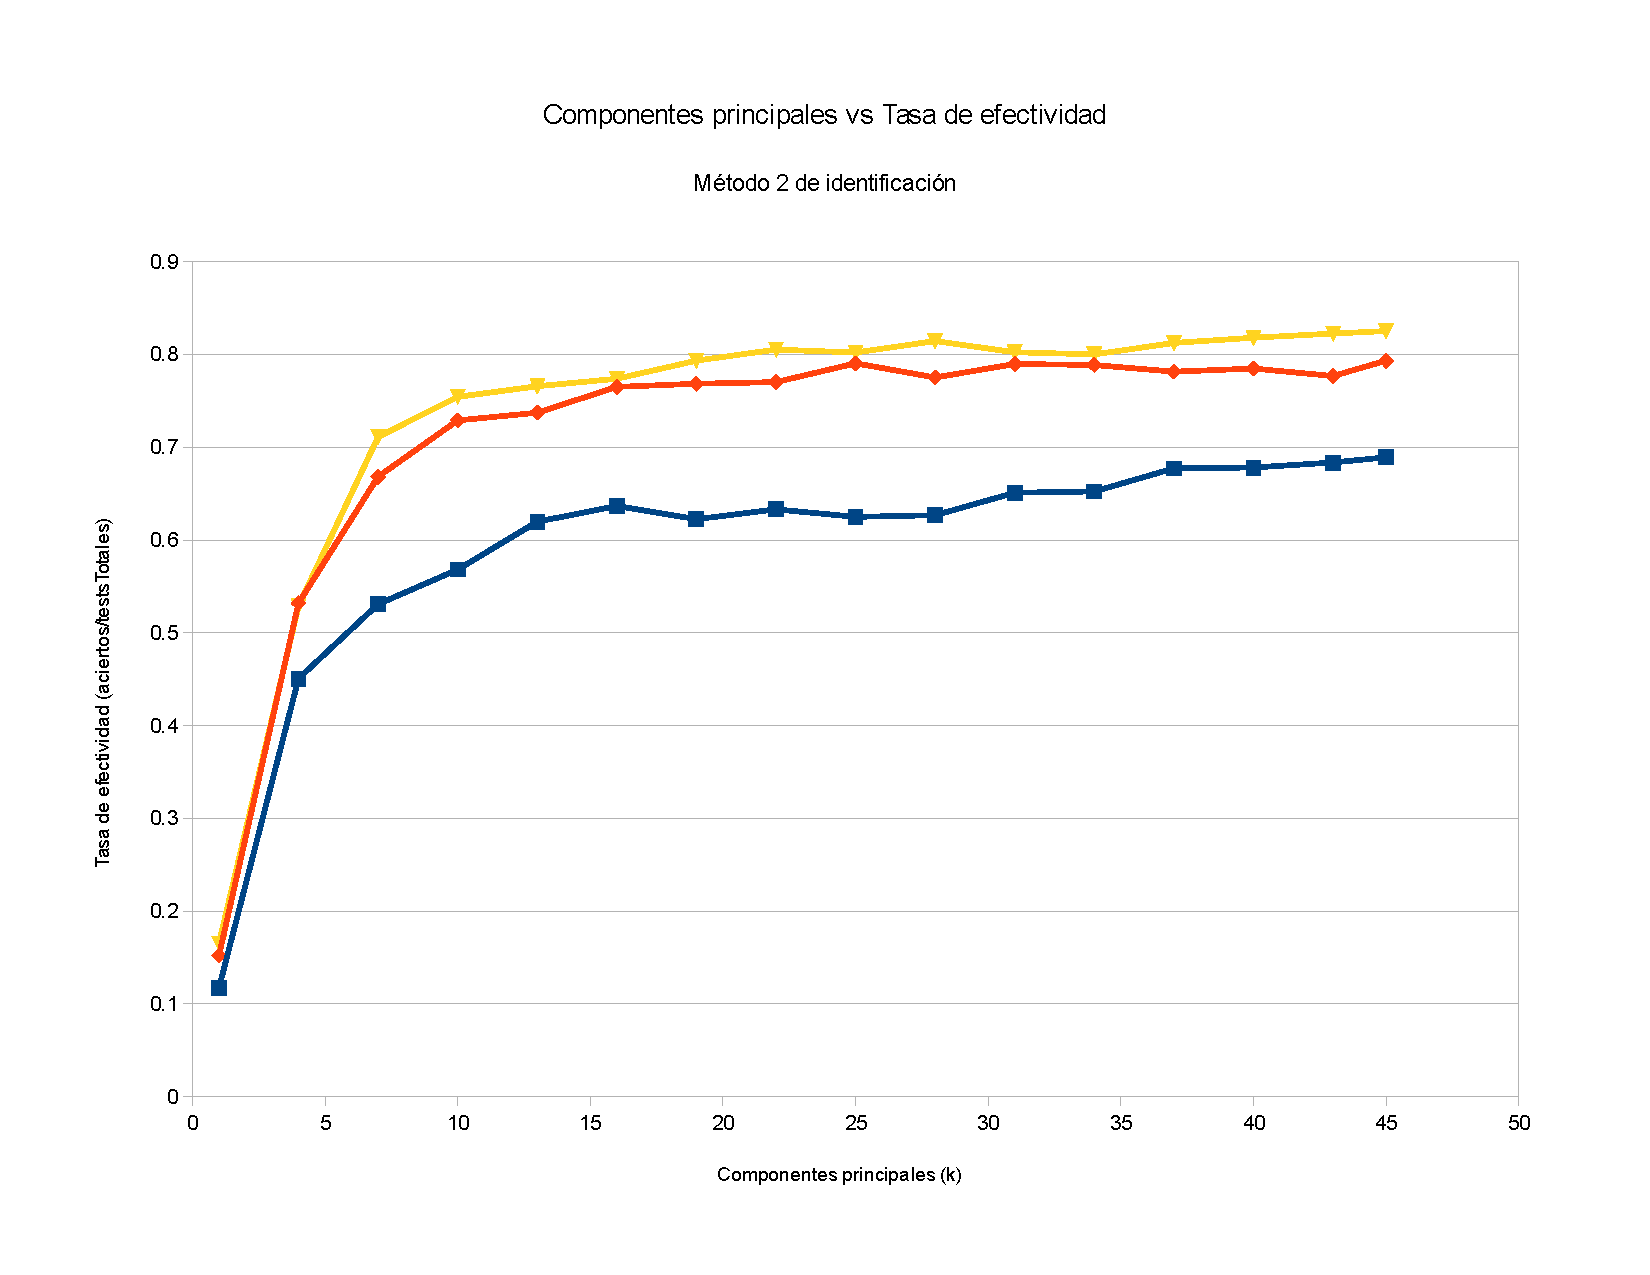
\includegraphics[scale=0.5]{graphs/componentesPrincipalesVsTasaDeEfectividadM2.pdf}
\caption{El método 2 de identificación se corresponde con el de Distancia Mínima Promedio}
\label{CPvsTE}
\end{figure}

Línea azul: $nimgp = 3$. Línea roja: $nimgp = 6$. Línea amarilla: $nimgp = 9$.
\newpage
\section{Discusión}
%Se incluirá aquí un análisis de los resultados obtenidos en la sección anterior (se analizará
%su validez, coherencia, etc.). Deben analizarse como míınimo los ítems pedidos en el
%enunciado. No es aceptable decir que “los resultados fueron los esperados”, sin hacer
%clara referencia a la teoría la cual se ajustan. Además, se deben mencionar los resul-
%tados interesantes y los casos “patológicos” encontrados.

\subsection{Análisis de resultados de tasa de efectividad en functión de las componentes principales}
Se ve claramente como la tasa de efectividad aumenta al incrementarse el número de componentes principales utilizadas. Éste es un comportamiento
que esperábamos. Sin embargo, nos sorprende cuán rápido disminuye la velocidad a la que crece la tasa de efectividad. Para $k = 12$ podemos ver
que ya alcanzamos un $90\%$ de la tasa de efectividad total que conseguimos hasta donde alcanzaron nuestros tests, $k = 45$. Incrementar las 
componentes principales a partir de ese momento logra aumentar la tasa de efectividad sólo un $10\%$ más. Éste comportamiento interpretamos
que se debe a que las primeras 12 componentes principales sintetizan el $90\%$ de la información. Se desprende de dicha interpretación
el grado de importancia que tiene calcular los autovalores en orden descendente por magnitud de su módulo. Si tenemos en cuenta que la matriz
podría llegar a tener $10304$ autovalores diferentes, dada la resolución de las imágenes, las 12 componentes principales representan
menos de un $0,2\%$ de las mismas.
\par
A nivel práctico podemos aconsejar que a menos que los requerimientos sobre la tasa de efectividad sean muy demandantes basta con 
tomar unas pocas componentes principales para lograr una buena tasa de efectividad.
\par
Finalmente, podemos observar que la forma de las 3 curvas es prácticamente igual, simplemente sufren un desplazamiento sobre el eje
vertical. Esto nos lleva a intuir que tomar mayores $nimgp$ nos provee una mayor tasa de efectividad sin necesidad de aumentar el $k$ que
utilizamos.

\subsection{Análisis de la tasa de eficiencia en función de la cantidad de personas}
Como se puede observar en los resultados la tasa de efectividad disminuye a medida que aumenta la cantidad de personas, posiblemente debido a que, como se mencionó anteriormente, la probabilidad de que haya más sujetos parecidos entre sí o imágenes similares de distintos sujetos. Además la probabilidad de aciertos es menor al aumentar la cantidad de sujetos, es decir, si hay 2 sujetos la probabilidad de acierto sin ningún tipo de información de $\frac{1}{2}$, en cambio con 10 sujetos es $\frac{1}{10}$, en general la probablidad de acertar sin ningún tipo de información es $\frac{1}{n}$ donde $n$ es la cantidad de personas. Sería interesante analizar el comportamiento asintótico del gráfico para hallar una cota inferior para la tasa de eficiencia y deducir si el algoritmo puede ser arbitrariamente malo. Lamentablemente solo se dispone de $40$ imágenes, por lo que solo podemos dar una aproximación de la tasa de eficiencia para $40$ o menos imágenes.

\subsection{Análisis de la tasa de efectividad en función de $nimgp$}
Lo primero que nos llama la atención de estos resultados es la gran diferencia que devuelve en la tasa de efectividad que se obtuvo
tomando $nimgp = 1$ y variando $k = 15, 30, 45$. No estamos seguros a qué se debe este comportamiento. Intuimos que como sólo se toma
una foto por sujeto para la base de entrenamiento los resultados dependen mucho de la foto que se toma. Se intentó reducir este tipo
de ruido realizando varias veces el mismo test con seleccionando aleatoriamente las imágenes y aparentemente no tuvimos éxito para
el caso más sensible.
\par
Se puede apreciar claramente como la tasa de efectividad aumenta a medida que incrementamos $nimgp$, comportamiento que predijimos, sin embargo,
no nos esperábamos que luego de cierto umbral la tasa de efectividad comience a decrecer. Sin tener en cuenta el caso $nimgp = 1$, vemos 
claramente que la curva sigue una forma de parábola abriéndose hacia abajo, alcandando su máximo en $nimgp = 6$. No estamos seguros
a qué se debe el decrecimiento que sufre la tasa de efectividad para valores $nimgp > 6$.

\subsection{Análisis de la tasa de eficiencia en función de la resolución de las imágenes}
Los resultados obtenidos si bien no son los que se esperaban implican ciertas cuestiones interesantes. Primero, la resolución de imágenes son prácticamente idénticas para todas las condiciones por lo que se puede suponer que para ambas resoluciones la información que contienen las imágenes es suficiente y necesaria para que el análisis de componentes principales funcione de la manera esperada. Si bien nuestra suposición inicial no era correcta, es decir que a una resolución mayor se obtiene una tasa más alta, el error partió de suponer que la resolución más chica era lo suficiente mala como para arrojar peores resultados. Este percepción errónea provino de que las imágenes chicas son algo más difícil (pero no imposible con un poco de tiempo) de identificar a simple vista (con la cantidad apropiada a zoom).

\subsection{Análisis de comparación de los métodos de identificación}
Vemos que las curvas tienen la misma forma que en la primera experimentación, lo cual nos dice que los dos métodos de identificación
se comportan de la misma forma ante la variación de la cantidad de componentes principales utilizadas. Además, se comportan de la misma
forma ante los cambios en $nimgp$ ya que las 3 curvas aparecen una sobre la otra en el mismo orden en los dos gráficos. Sin embargo, 
podemos ver que para el método de identificación por distancia mínima las curvas roja y amarilla, correspondientes a $nimgp = 6$ y $nimgp = 9$
respectivamente, a partir de $k = 10$ obtienen tasas de efectividad superiores a $0.8$. En cambio, para el método de distancia promedio mínima
a penas superan la tasa de efectividad $0.8$. Concluimos que el método de identificación por distancia mínima alcanza una mayor tasa de 
efectividad utilizando la misma cantidad de componentes principales y valores de $nimgp$. Sugerimos utilizar éste método para cualquier
aplicación práctica por sobre el de distancia promedio mínima.


\newpage
\section{Conclusiones}
%Esta sección debe contener las conclusiones generales del trabajo. Se deben mencionar
%las relaciones de la discusión sobre las que se tiene certeza, junto con comentarios
%y observaciones generales aplicables a todo el proceso. Mencionar también posibles
%extensiones a los métodos, experimentos que hayan quedado pendientes, etc.


\newpage
\section{Apéndices}
\include{demo}
%En el apéndice A se incluirá el enunciado del TP. En el apéndice B se incluirán los
%códigos fuente de las funciones relevantes desde el punto de vista numérico. Resultados
%que valga la pena mencionar en el trabajo pero que sean demasiado específicos para
%aparecer en el cuerpo principal del trabajo podrán mencionarse en sucesivos apéndices
%rotulados con las letras mayusculas del alfabeto romano. Por ejemplo: la demostración
%de una propiedad que aplican para optimizar el algoritmo que programaron para resolver
%un problema.




\newpage
%\section{Referencias}
%Es importante incluir referencias a libros, artículos y páginas de Internet consultados
%durante el desarrollo del trabajo, haciendo referencia a estos materiales a lo largo del
%informe. Se deben citar también las comunicaciones personales con otros grupos.
\addcontentsline{toc}{section}{Referencias}
\begin{thebibliography}{1}
\bibitem{burden} Richard Burden. \textbf{Numerical Analysis.}  Brooks Cole, 2000.
\end{thebibliography}




\end{document}
